\section{Source Code Analysis}
\label{source-code-analysis}

Data la complessità dei moderni sistemi software, la presenza di strumenti per
il supporto alla creazione e alla manutenzione di questi è fondamentale. Da
questa riflessione emergono le ragioni che portano all’interesse della comunità
informatica per strumenti di source code analysis. Strumenti di questo tipo sono
infatti in grado di fornire informazioni di estrema importanza agli sviluppatori
di un sistema, informazioni che possono essere utilizzate da questi per
coordinare il proprio lavoro e aumentare la produttività complessiva.

Nella letteratura, la \textit{source code analysis} viene definita come il
processo di estrazione di un informazioni riguardo ad un programma a partire
dall'analisi del codice sorgente di questo. \cite{DBLP:journals/jss/DeanHKV06}

La precedente definizione fa riferimento a due diversi concetti, il concetto di
codice sorgente e il concetto di analisi.

Nel contesto della source code analysis, il termine codice sorgente viene
utilizzato, soprattutto nella letteratura, per indicare una descrizione del
comportamento di un programma in un formato testuale, statico, leggibile e
partire dalla quale è possibile produrre una versione del sistema software
completamente eseguibile. Questa definizione è costruita in maniera tale da
includere i codici macchina, linguaggi di alto livello e anche rappresentazioni
grafiche eseguibili di un sistema.

Il termine analysis viene invece utilizzato per indicare una qualsiasi procedura
automatica o semi-automatica che produce nuova conoscenza rispetto ad un sistema
a partire dal codice sorgente di questo. \cite{DBLP:conf/icse/Binkley07}

Nella letteratura, la source code analysis viene spesso spesso accorpata al
settore che si occupa della manipolazione di codice sorgente, è viene utilizzata
la sigla SCAM, Source Code Analysis and Manipulation, per riferirsi a questo
particolare ambito di ricerca. \cite{DBLP:conf/scam/2001}

In questo contesto, il termine “manipolazione" viene utilizzato per indicare una
qualsiasi procedura automatica o semi-automatica che produce codice sorgente a
partire da codice sorgente.

Come accennato in apertura di questa sezione, la source code analysis ricopre un
ruolo di grande importanza nel contesto dell'ingegneria del software, tanto che
applicazioni di tecniche di SCAM possono essere rintracciate in diverse fasi
del ciclo di vita di un sistema software.

Dal supporto per la creazione di un programma all’interno di un IDE, alla
compilazione e deployment, al supporto per l'identificazione e correzione di
errori durante la manutenzione, in ciascuno di questi contesti vengono
utilizzate tecniche di Source Code Analysis.

Un altro aspetto che contribuisce a rendere importante questo ambito di ricerca
è rappresentato dalla significatività e onnipresenza del soggetto a cui questa
si riferisce: il codice sorgente.

Il progetto di un sistema software ha solitamente inizio con la costruzione di
un modello del funzionamento di questo, come ad esempio diagrammi prodotti
utilizzando il linguaggio di modellazione UML. Questi modelli consentono la
rappresentazione del sistema ad un livello di astrazione alto e gestibile in
modo semplice e veloce. Tuttavia, nelle fasi successive del processo questi
modelli dovranno necessariamente essere \enquote{\textit{compilati}} utilizzando
una rappresentazione che vive ad un livello di astrazione inferiore: il codice
sorgente.

Sfortunatamente, una diretta implementazione dei modelli precederete citati
porta alla creazione di codice tipicamente incompleto e che per questa ragione
richiede aggiunte e modiche. Aggiunte e modifiche impossibili da prevedere al
momento della costruzione dei modelli, in quanto molto spesso relative a
dettagli implementativi, e che rappresentano quindi un inevitabile effetto
collaterale dell'attività di sviluppo. Queste modifiche portano alla presenza di
incongruenze tra modelli e codice sorgente ed è proprio la presenza di queste
incongruenze a rendere il codice sorgente l’unica sorgente di informazioni
realmente attendibile rispetto all’effettivo funzionamento di un sistema
software.

Questa sottosezione ha fornito una definizione di source code analysis, allo
scopo di indicare l'ambito di ricerca all'interno del quale lo strumento
discusso da questa tesi si colloca. Ha cercato inoltre di sottolineare
l'importanza di questo ambito di ricerca nel contesto del più ampio campo
dell'ingegneria del software. Nella prossima sottosezione, viene approfondita la
struttura di uno strumento di source code analysis, in maniera tale da fornire
al lettore una panoramica rispetto alla tipologia di strumenti che CLAST
consente di creare.

\subsection{Struttura di uno strumento di Source Code Analysis}
\label{sca-architecture}

I prossimi paragrafi descrivono le tre componenti fondamentali di un
tradizionale sistema per la source code analysis. Queste componenti sono
rappresentate da:

\begin{itemize}

\item un parser per il codice sorgente del sistema in analisi;

\item una struttura dati per la rappresentazione interna allo strumento del
codice sorgente parsato;

\item un meccanismo che operi la reale analisi del sistema a partire dalla
rappresentazione interna.

\end{itemize}

La prima componente, il parser, opera un'elaborazione del codice sorgente al
fine di produrre una o più rappresentazioni del sistema che si desidera
analizzare utilizzando la struttura dati per la rappresentazione del sistema
specifica dello strumento. In sostanza, questo passo opera la conversione dalla
sintassi concreta, utilizzata dal codice sorgente vero e proprio, ad una
sintassi astratta, che meglio si presta alla particolare analisi che si desidera
operare.

La grande maggioranza degli strumenti per la source code analysis fa uso del
parser integrato al compilatore per il linguaggio di programmazione utilizzato
per la costruzione del sistema in analisi. Parser di questo tipo consentono
l’elaborazione dell’intero linguaggio di programmazione. Tuttavia, nel caso in
cui solamente un sottoinsieme della sintassi concreta di un linguaggio sia di
reale interesse per l’analisi, vengono solitamente utilizzate tecniche più
semplici.

La tendenza è quindi quella ad operare un riutilizzo di parser già esistenti. La
definizione manuale di un parser risulta molto spesso un'attività
particolarmente impegnativa nel processo di costruzione di uno strumento di
source code analysis. La complessità dei linguaggi di programmazione porta
infatti molto spesso a significative difficoltà nella realizzazione di questa
componente; nonostante si tratti di un procedimento semplice dal punto di vista
concettuale responsabile solamente per la semplice lettura e trasformazione di
un testo.

La seconda componente di uno strumento per la source code analysis è
rappresentata dalla struttura dati interna utilizzata per la modellazione del
sistema in analisi. La grande maggioranza delle tecniche di rappresentazione e
strutture utilizzate dagli strumenti di source code analysis prende ispirazione
dal, o fa riferimento al, mondo dei compilatori. Questo perché la quasi totalità
dei compilatori prevede una fase che si pone come obiettivo proprio quello che
il componente analizzato in questo paragrafo si pone: la trasformazione di un
programma in una rappresentazione maggiormente adatta all’analisi da parte di
uno strumento automatico. In particolare però, una trasformazione che conservi
le proprietà significative per il dominio di interesse dell'analisi ma che sia
maggiormente specifica rispetto al dominio di interesse.

Diverse tecniche e strutture per la rappresentazione interna ad uno strumento
vengono utilizzate da differenti strumenti di source code analysis. Alcuni
esempi di strutture per la rappresentazione del codice sorgente sono
rappresentati da control-flow graphs, call graphs e abstract syntax trees.

In alcuni casi la produzione di queste rappresentazioni interne può essere
compiuta direttamente dalla componente parser dello strumento di source code
analysis. In altri casi, specialmente in contesti più complessi, sono invece
necessarie ulteriori analisi al fine di produrre una rappresentazione definitiva
che possa effettivamente essere utilizzata dalla componente di analisi.

Infine, la terza ed ultima componente di uno strumento di source code analysis è
rappresentata dall’effettivo analizzatore.

Nel corso degli anni sono state definiti e impiegati una grande quantità di
meccanismi e tipi di analisi del codice sorgente. Un approfondimento di ciascuno
di questi esula dagli obiettivi di questa tesi. All’interno del Capitolo
\ref{applications} di questa tesi, verranno però analizzati i principali, e
anticipati, tipi di analisi che la rappresentazione offerta dalla libreria CLAST
consente con maggiore dettaglio.

Dopo aver presentato le principali componenti per la creazione di uno strumento
di source code analysis, la Sottosezione \ref{sca-approches} approfondisce i
principali approcci alla creazione di uno strumento di questo tipo.

\begin{figure}
\makebox[\textwidth][c]{
  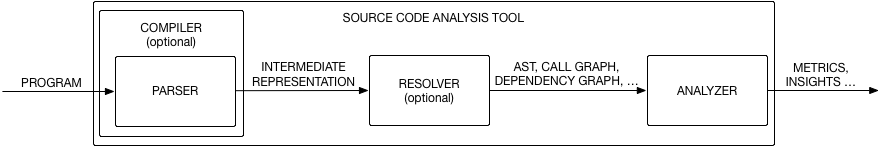
\includegraphics[scale=0.5]{img/sca-tool-architecture}
}
\caption{Architettura di uno strumento di Source Code Analysis}
\label{fig:sca-tool-architecture}
\end{figure}

Nel contesto dell'architettura appena illustrata, mostrata grafica in Figura
\ref{fig:sca-tool-architecture} la libreria CLAST, soggetto di questa tesi, va a
definire sia la prima componente, un parser per il linguaggio di programmazione
Common Lisp, sia la seconda componente, ossia una struttura dati organizzata in
forma di AST che raccoglie il maggior numero possibile di informazioni
disponibili rispetto al codice del sistema in analisi. I dettagli relativi della
progettazione ed implementazione di queste componenti verranno approfonditi nel
corso dei prossimi capitoli di questa tesi.

La libreria ha quindi lo scopo di semplificare la creazione di strumenti per la
source code analysis fornendo quelle componenti comuni a qualsiasi strumento di
source code analysis per il linguaggio Common Lisp; dando la possibilità ad uno
sviluppatore di concentrarsi sulla definizione di un analizzatore specifico per
i contenuti e le metriche di interesse, senza la necessità di dover definire
l'infrastruttura di analisi che sarebbe altrimenti obbligato a costruire.

\subsection{Approcci per la costruzione di uno strumento di Source Code
Analysis}
\label{sca-approches}

Gli attuali strumenti di source code analysis sono sviluppati utilizzando
principalmente due diverse strategie di sviluppo. Alcuni strumenti realizzano
direttamente la fase di parsing del codice sorgente del sistema in analisi.
Strumenti di questo tipo prevedono quindi una componente parser al loro interno,
componente che deve essere sviluppata e manutenuta parallelamente allo strumento
stesso. Un approccio opposto a quello appena descritto è rappresentato dalla
costruzione di strumenti che operano a partire da uno o più strumenti già
disponibili, come ad esempio un compilatore in grado di produrre l'abstract
syntax tree associato ad un programma e esporlo attraverso un’API.

In seguito vengono discussi questi due approcci, indicando vantaggi e
svantaggi, problemi e sfide caratteristici di ciascuno di questi. Questo al
fine di presentare al lettore con maggiore chiarezza il contesto di risorse
all’interno del quale, uno strumento come quello descritto da questa tesi, si
colloca dal punto di vista dello sviluppo e delle risorse preesistenti.

Dal punto di vista pratico, la scelta più condizionante per il progettista di
uno strumento per la source code analysis è la seguente: sviluppare
parallelamente al proprio strumento un parser per il linguaggio, o i linguaggi,
di programmazione di riferimento oppure dipendere da un parser già disponibile.

Lo sviluppo dell’intera infrastruttura necessaria per la creazione dello
strumento che si desidera produrre, compreso un parser, ha alcuni vantaggi. In
prima battuta, lo sviluppo del nuovo parser e le attività svolte da questo
potrebbero essere limitate ad un sottoinsieme del linguaggio di riferimento e di
conseguenza ad un sottoinsieme della grammatica di questo. Questo porta ad
ottenere un componente più leggero e facilmente integrabile all'interno
dell'architettura dello strumento che si desidera produrre.

Questo approccio può richiedere la disponibilità di un’infrastruttura per lo
sviluppo di un parser, come ad esempio lexers, generatori di parser e altro
ancora, ma, quanto meno, necessità di un grammatica per il linguaggio che si
desidera analizzare. Uno dei problemi più comuni in questo contesto è che molto
spesso l’implementazione di un linguaggio e la grammatica utilizzata per
descriverlo non sono perfettamente corrispondenti. In altri casi invece la
grammatica è incompleta, come ad esempio è stato per lungo tempo nel caso del
linguaggio di programmazione C++, la cui grammatica non faceva riferimento al
costrutto template presente in questo, oppure la grammatica potrebbe non essere
completamente compatibile con i differenti dialetti di un linguaggio.

Un passo che consente una semplificazione di questo processo può essere
rappresentato dall'estensione o aggiornamento una grammatica già esistente.
Questo al fine di non dover necessariamente definire una formalizzazione
completamente nuova dell'intera grammatica di un linguaggio di programmazione.
La scrittura di una nuova grammatica può essere estremamente dispendiosa; il
risultato può essere incompleto, poco robusto, o addirittura accettare un
sovrainsieme del linguaggio. In ogni caso, la continua evoluzione che
caratterizza la maggioranza dei linguaggio di programmazione di attualità
implica la necessità di costanti aggiornamenti della grammatica sviluppata, un
compito molto spesso non banale.

Fortunatamente, grammatiche precise, robuste e aggiornate, così come parser per
queste, sono solitamente incorporate nel compilatore per il linguaggio di
programmazione di interesse e, molto spesso, vengono rese disponibili
all’utilizzo esterno al compilatore stesso. La maggioranza dei frontend dei
compilatori per linguaggi di programmazione attuali può infatti essere estesa
allo scopo di consentire l’analisi e l’estrazione di informazioni dal codice
sorgente fornito in input al compilatore. \cite{gregor2012}

In contesti di questo tipo, la maggiore difficoltà è però rappresentata dal
fatto che gli obiettivi di un compilatore e di uno strumento per la source code
analysis sono differenti e, in molti casi, in contrasto.

Lo scopo di un compilatore è infatti quello di produrre codice eseguibile, a
partire dal codice sorgente in input, che sia il più efficiente possibile e con
il minor impiego di risorse possibile. Lo scopo di uno strumento per la source
code analysis è invece quello di produrre la rappresentazione più ricca
possibile del codice sorgente in input rispetto ai particolari parametri di
interesse all’analisi.

Per questa ragione, a seconda del compilatore e a seconda dell’API offerta da
questo, è possibile seguire due strade distinte per poter costruire uno
strumento per la source code analysis a partire da questo:

\begin{itemize}

\item apportare una modifica al compilatore stesso, in maniera tale che sia
possibile l'accesso alla rappresentazione da parte di strumenti esterni a
questo;

\item costruire un wrapper per le funzionalità interessanti offerte dal
compilatore. Nel caso in cui il compilatore memorizzi una rappresentazione del
codice sorgente del programma in input, ad esempio in forma di AST, come formato
di rappresentazione intermedia prima della generazione di codice macchina, è
possibile costruire un analizzatore che lavori a partire da questa
rappresentazione, senza la necessità di operare modifiche al compilatore stesso.
Tuttavia, qualora l’accesso ai formati di rappresentazione intermedi non fosse
disponibile all’esterno, sarebbe però comunque necessario operare un modifica
del codice del compilatore in maniera tale da rendere questa esportazione
possibile.

\end{itemize}

\begin{figure}
\makebox[\textwidth][c]{
  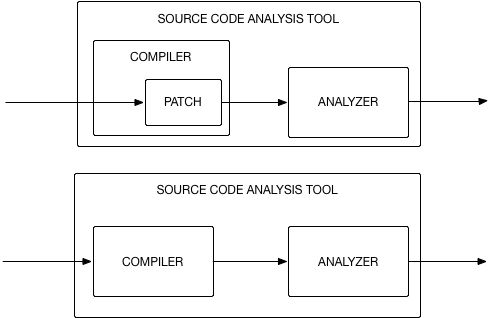
\includegraphics[scale=0.5]{img/sca-compiler-strategies}
}
\caption{Strategie per la strutturazione dell'interazione tra uno strumento di
source code analysis e un compilatore}
\label{fig:sca-compiler-strategies}
\end{figure}

Uno degli svantaggi principali del primo approccio citato è rappresentato dal
fatto che, in molti casi, l'architettura del compilatore non viene definita in
maniera tale da facilitare o consentire l'estensione che porta alla produzione
della rappresentazione del sistema utilizzata internamente dal compilatore
stesso. Ciò rende particolarmente complesse le attività di implementazione
dell'estensione. Inoltre, un progetto che include l'estensione di un compilatore
richiede necessariamente una fase di studio e comprensione del funzionamento
interno di questo, attività spesso non triviali.

Uno degli svantaggi principali del secondo approccio è invece rappresentato dal
fatto che, anche strutturando la modifica operata al compilatore in maniera tale
da essere il meno dipendente possibile dalle peculiarità di questo, è sempre
possibile che una nuova versione del compilatore renda le modifiche
precedentemente operate incompatibili, portando a dover riscrivere gran parte
dello strumento. Una seconda problematica significativa che caratterizza il
secondo approccio citato è rappresentata dal fatto che, come riportato in
precedenza, lo scopo di un compilatore e di uno strumento per la source code
analysis sono fondamentalmente diversi e, per questa ragione, è molto probabile
che la rappresentazione che il compilatore offre del codice sorgente, ad esempio
attraverso i nodi di un AST, non riporti informazioni che sarebbero invece di
interesse per lo strumento e, viceversa, riporti una grande quantità di
informazioni di scarso, se non inesistente, interesse per lo strumento. Aspetto
che porta alla necessità di introdurre un fase di aggiunta o rimozione di
elementi dalla rappresentazione fornita dal compilatore, aumentando la
complessità dello strumento.

Sfortunatamente nessuno dei compilatori attualmente disponibili per il
linguaggio di programmazione Common Lisp fornisce un'API che consenta di
sfruttare la rappresentazione interna che ciascuno di questi produce durante la
propria elaborazione. Inoltre, la presenza di differenti implementazioni del
linguaggio e la grande frammentazione della comunità Lisp derivata da questa,
rendono impossibile utilizzare un approccio di estensione di un compilatore.
Infatti, i vantaggi legati alla possibilità di utilizzare uno strumento source
code analysis costruito attraverso l'estensione di un particolare compilatore
sarebbe limitata solamente alla ristretta porzione di utenti di quella
particolare implementazione.

Si è pertanto scelto di seguire una via diversa, sfruttando la strutturazione
del linguaggio Common Lisp, già molto prossima alla struttura di un AST, e
godendo della possibilità di definire un meccanismo di rappresentazione non
condizionato dalle necessità di un compilatore, andando a strutturare CLAST come
uno strumento completamente distinto da un compilatore e implementando quindi
autonomamente le strutture necessarie per la creazione di strumenti di source
code analysis per il linguaggio Common Lisp.

Questa sezione ha presentato il campo della source code analysis, ossia l'ambito
di ricerca all'interno del quale questa tesi si colloca, fornendo al lettore
alcuni spunti per comprendere l'importanza che questa ricopre all'interno del
più generale campo dell'ingegneria del software. Si è inoltre presentata la
tradizionale architettura di uno strumento di source code analysis e i
principali approcci alla costruzione di strumenti di questo tipo. Questo al fine
di illustrare la collocazione della libreria CLAST e l'architettura fondamentale degli strumenti all'interno dei quali questa andrebbe ad inserirsi.
